\uuid{kk4y}
\exo7id{5538}
\auteur{rouget}
\organisation{exo7}
\datecreate{2010-07-15}
\isIndication{false}
\isCorrection{true}
\chapitre{Courbes planes}
\sousChapitre{Propriétés métriques : longueur, courbure,...}

\contenu{
\texte{
Soit $(\Gamma)$ la courbe d'équation $y=\ln(\cos x)$, pour $-\frac{\pi}{2}<x<\frac{\pi}{2}$. Calculer l'abscisse curviligne $s$ quand $O$ est l'origine des abscisses curvilignes et l'orientation est celle des $x$ croissants. Trouver une relation entre $R$ et $s$. Tracer $(\Gamma)$ et sa développée.
}
\reponse{
$\mathcal{C}$ est le support de l'arc paramétré $t\mapsto\left(
\begin{array}{c}
t\\
\ln(\cos t)
\end{array}
\right)$.

\begin{center}
$\overrightarrow{\frac{dM}{dt}}=\left(
\begin{array}{c}
1\\
-\sin t/\cos t
\end{array}
\right)=\frac{1}{\cos t}\left(
\begin{array}{c}
\cos t\\
-\sin t
\end{array}
\right)$.
\end{center}
Puisque $\frac{1}{\cos t}>0$ et que $\left(
\begin{array}{c}
\cos t\\
-\sin t
\end{array}
\right)$ est unitaire, on a successivement $\frac{ds}{dt}=\frac{1}{\cos t}$, $\overrightarrow{\tau}(t)=\left(
\begin{array}{c}
\cos t\\
-\sin t
\end{array}
\right)$, $\overrightarrow{n}(t)=\left(
\begin{array}{c}
\sin t\\
\cos t
\end{array}
\right)$, $\alpha(t)=-t$ puis

\begin{center}
$R(t)=\frac{ds/dt}{d\alpha/dt}=-\frac{ds}{dt}=-\frac{1}{\cos t}$.
\end{center}
Ensuite, si $s$ est l'abscisse curviligne d'origine $0$ orientée dans le sens des $t$ croissants,

\begin{center}
$s(t)=\int_{0}^{t}s'(u)\;du=\int_{0}^{t}\frac{1}{\cos u}\;du=\ln\left|\tan\left(\frac{t}{2}+\frac{\pi}{4}\right)\right|$.
\end{center}
Enfin,

\begin{center}
$\Omega(t)=M(t)+R(t)\overrightarrow{n}(t)=\left(
\begin{array}{c}
t\\
\ln(\cos t)
\end{array}
\right)-\frac{1}{\cos t}\left(
\begin{array}{c}
\sin t\\
\cos t
\end{array}
\right)=\left(
\begin{array}{c}
t-\tan t\\
\ln(\cos t)-1
\end{array}
\right)$.
\end{center}

$$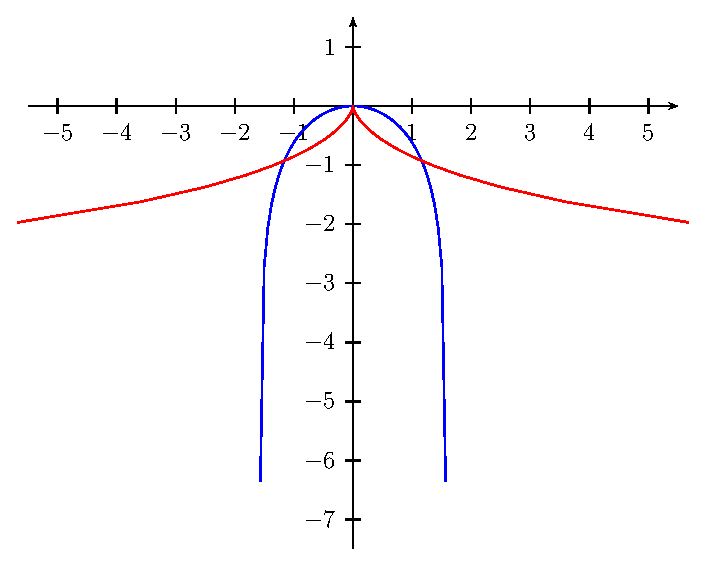
\includegraphics{../images/img005538-1}$$
}
}
